\section{Theoretical aspects}

\emph{%
% 
This section treats the fundamentals of the theory of particle physics.
% 
Only topics that are deemed relevant for the rest of this thesis are treated, and as such this section is by no means comprehensive.
%
First the standard model and its particles are generally introduced, followed by \tk{todo}.
% 
For a more comprehensive, accessible overview of particle physics, the reader is referred to Ref.~\cite{griffiths}, and for mathematical formulations of underlying symmetries and the derivations of the Feynman rules to Ref.~\cite{peskin}.
}

% ____________________________________________________________________________
\subsection{The standard model}

The standard model (SM), widely recognized as one of the greatest successes of particle physics, is the physics model that summarizes, to the best of our knowledge, the particles that exist in nature, and how they interact with one another.
% 
Its predictions are consistent with many experiments performed in the second half of the 20${}^\text{th}$ century at scales extending over several orders of magnitude.
% 
The discovery~\cite{Aad:2012tfa,Chatrchyan:2012xdj,Chatrchyan:2013lba} of a particle compatible with the SM Higgs boson at the CERN LHC completed an important of the puzzle of the SM, the mechanism behind the masses of the intermediate vector bosons.
% 
Its conception is the result of decades of monumental effort from both the experimental and theoretical particle physics communities.


The SM is a quantum field theory (QFT); more specifically, it is a \textit{renormalizable} and \textit{locally invariant gauge theory}, meaning the fields $\psi$ are invariant under local gauge transformations.
% 
Its particles and interactions are encapsulated in the \textit{SM Lagrangian density} $\lagrangiansm$ (from here on referred to as simply the \textit{SM Lagrangian}), whose full, lengthy description can be found in Ref.~\cite{todo}.
% 
The SM Lagrangian fulfills the requirements of local gauge invariance and renormalizability, but it is by no means the only Lagrangian to do so.
% 
The form of the SM Lagrangian is `derived' (not in the mathmatical sense) from our knowledge of non-relativistic quantum mechanics, symmetry considerations, and from experiment.
% 
It is not a result of some underlying principles of QFT; it is instead postulated in such a way to fit experimental observations.


In principle, deriving the physics of electromagnetic, strong, and weak interactions is then as simple as solving the equation of motion, which much like in classical mechanics is derived from the least-action principle:
% 
\begin{linenomath*}
\begin{equation}
\label{eq:eom}
\partial_\mu \left(
    \frac{
        \partial \lagrangian
        }{
        \partial \left( \partial_\mu \psi \right)
        }
    \right)
    -
    \frac{\partial\lagrangian}{\partial\psi}
    = 0
\end{equation}
\end{linenomath*}
% 
where $\mu$ is in index to the four dimensions of spacetime, $\partial_\mu$ is shorthand for $\frac{\partial}{\partial x^\mu}$, i.e. the spacetime derivative with respect to the coordinate $x^\mu$, and $\psi$ (shorthand for $\psi(x^\mu)$) is a field.
% 
For a theory with multiple fields (as is the case for the SM), Equation~(\ref{eq:eom}) is supposed to hold for each field individually.
% 
Unfortunately, there is no easy solution to the equation of motion of the SM Lagrangian, and we need to resort to perturbative expansion to find approximate solutions, which is no trivial matter even for the simplest of particle physics processes.
% 
The full treatment of this perturbative expansion is beyond the scope of this text, and the reader is referred to the excellent treatment of this topic in Ref.~\cite{peskin}.
% 
In short, the perturbative expansion can be simplified to a sum of wonderfully descriptive \textit{Feynman diagrams}, which represent the terms of the perturbative expansion, and the \textit{Feynman rules}, which map the diagrams to an evaluable formulaic form.


Although undeniably a great success, the SM comes with a number of important `gaps'.
% 
For example, it lacks a description of gravity, highlighting the largest incompatibility of the SM with the theory of general relativity.
% 
Furthermore, a description of dark matter and energy is lacking, and the observed matter-antimatter imbalance in the universe is also unexplained.
% 
These problems highlight some gaps in our description of naturally observed phenomena, but also on a more theoretical level there are aspects of the SM that are, for lack of a better word, uncomfortable.
% 
Overlooking for the moment the problem of massive neutrinos, the SM Lagrangian has 19 parameters that are, to the best of our knowledge, arbitrary.
% 
Although their experimentally determined values are used in SM predictions, there is no satisfying underlying theory explaining these parameters, which include for example the quark and lepton masses and the coupling constants of the electromagnetic, strong, and weak interactions.
% 
Given that the universe would look profoundly different under reasonably small variations of the values of these parameters~\cite{Cahn:1996ag}, it is a big open question how the parameters ended up having the values they have.
% 
% In fact, it is not even understood why there are 3 generations of leptons and quarks, rather than just 1, or any other number.


The particles encoded in SM Lagrangian can be categorized into quarks, leptons, gauge bosons, and the Higgs boson.
% 
The quarks come in 6 flavors, which are further categorized into 3 generations: the up and the down quark (the first generation), the strange and the charm quark (the second generation), and the bottom and the top quark (the third generation).
% 
The up, charm, and top quarks carry an electric charge $q = 2/3e$ (where $e$ is the elementary electric charge), whereas the down, strange, and bottom quarks carry $q=-1/3$.
% 
Each quark comes in 3 `colors', typically denoted red, blue and green; the color of a quark is to be understood as yet another property of the quark, and has nothing to do with the notion of color in colloquial use.
% 
Every quark has a corresponding antiquark which comes in 3 anticolors and carries an opposite electric charge.
% 
The leptons come in 3 generations as well: the electron $\electron^-$, the muon $\muon^-$ and the tau $\taulepton^-$, and their associated neutrinos, $\neutrino_\electron$, $\neutrino_\muon$, and $\neutrino_\taulepton$ respectively.
% 
The corresponding antileptons carry opposite electric charge; the antiparticle of the electron is typically referred to as a \textit{positron}.
% 
The gauge bosons are the mediators of the three fundamental forces in the SM---the photon being the mediator of the electromagnetic interaction, the vector bosons $\wboson^+$, $\wboson^-$, and $\zboson$ the mediators of the weak interaction, and the gluon $\gluon$ (of which there are 8) the mediator of the strong interaction.
% 
The final particle is the Higgs boson, unlike the other bosons a spin-0 particle, which through the Higgs mechanism gives the vector bosons their mass.
% 
All the SM particles are summarized once more in Fig.~\ref{fig:particles}.

\begin{figure}[hbtp]
  \begin{center}
    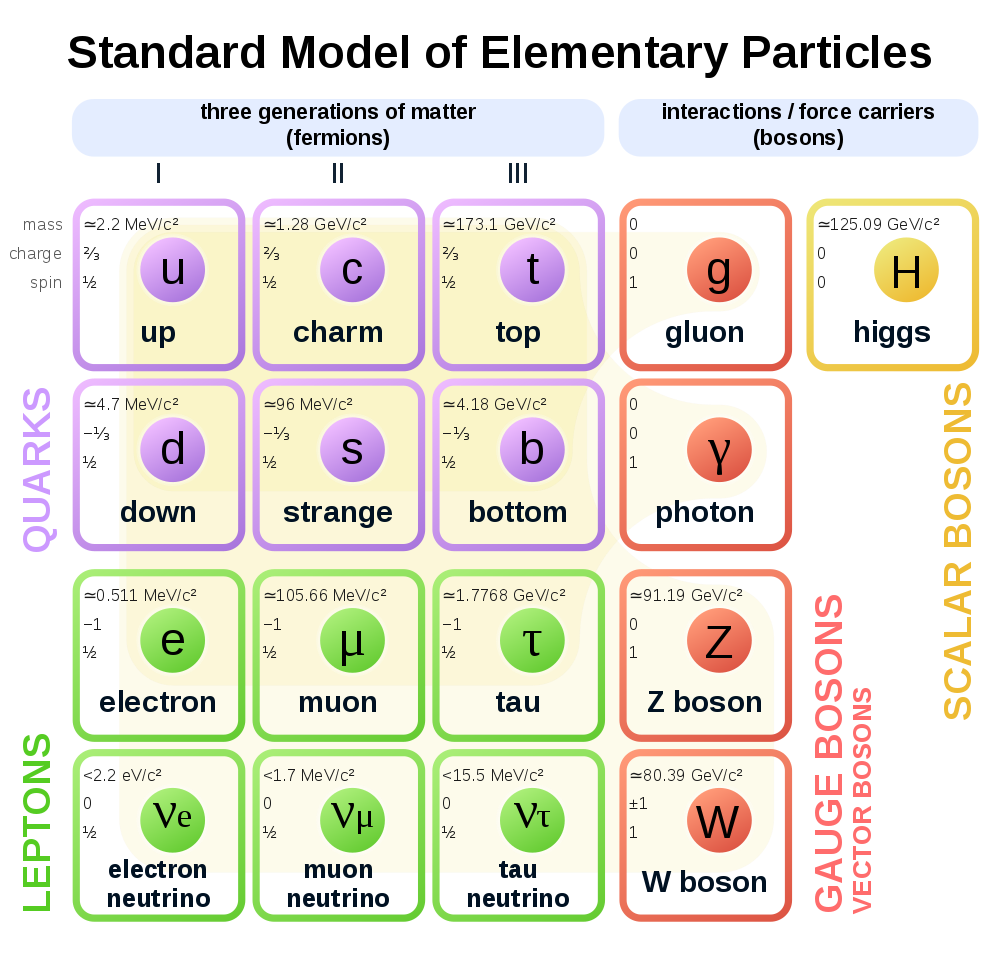
\includegraphics[width=0.7\linewidth]{img/theory/particles.png}
    \caption{
        Summary of the particles in the SM.
        % 
        THe quarks, leptons, gauge bosons and the Higgs boson are displayed in purple, green, red and yellow cells, respectively, sorted along generations for the fermions.
        % 
        Each cell contains three numbers in the top-left corner, corresponding to the mass, electric charge, and spin of the particle.
        % 
        Taken from Ref.~\cite{particles-wikicommons}.
        }
    \label{fig:particles}
  \end{center}
\end{figure}




% ____________________________________________________________________________
\subsection{Quantum chromodynamics}

\textit{%
The development of the theory of quantum chromodynamics has a fascinating history; at the time that quarks were first postulated by Gell-Mann and Zweig~\cite{todo}, there had been no experimental evidence for their existence at all.
% 
Only once deep inelastic electron-nucleon scattering became possible at sufficiently high energy to probe the internal structure of nucleons, the quark model was confirmed experimentally.
% 
This section starts from the full theory of QCD, loosely following the reasoning from Ref.~\cite{dissertori}, and mostly overlooks what was needed to develop it.
% 
For a historical overview of QCD the reader is referred to Refs.~\cite{dissertori,griffiths}. 
}


The SM Lagrangian for QCD is~\cite{dissertori}
% 
\begin{linenomath*}
\begin{equation}
\label{qcdlagrangian}
\lagrangian_\text{QCD} =
- \frac{1}{4} F^a_{\mu\nu} F^{a\mu\nu} 
+ \sum_\qquark \left( 
    \overline{\qquark}_i \mathrm{i} \gamma^\mu \delta_{ij} \partial_\mu \qquark_j
    - m_\qquark \delta_{ij} \overline{\qquark}_i \qquark_j
    - g_s \overline{\qquark}_i \gamma^\mu T_{ij}^a A_\mu^a \qquark_j
    \right)
\,,
\end{equation}
\end{linenomath*}
% 
where $\qquark$ ($\overline{\qquark}$) are the six (anti)quark fields, $\gamma$ are the gamma matrices, $m_\qquark$ is the mass of the quark, $F^a_{\mu\nu}$ is the gluon field strength tensor, $g_s$ is the coupling constant for QCD, $A^\mu$ are the gauge (gluon) fields, and $T^a$ are generators of the SU(3) gauge symmetry group, which in the matrix representation equal $\lambda^a/2$, $\lambda_a$ being the Gell-Mann matrices.
% 
The field strength tensor is given by
% 
\begin{linenomath*}
\begin{equation}
F^a_{\mu\nu}
    = \partial_\mu A^a_\nu - \partial_\nu A^a_\mu - g_s f^{abc} A_\mu^b A_\mu^c
\,,
\end{equation}
\end{linenomath*}
% 
where $f^{abc}$ are the structure constants of the SU(3) symmetry group.
% 
The first, gluonic part of Equation~(\ref{qcdlagrangian}) is responsible for the gluon self-interactions, which consist of a vertex with three gluons and a vertex with four gluons.
% 
The last part describes the interaction between quarks and gluons.


Besides the quark masses, the only free parameter in Equation~(\ref{qcdlagrangian}) is $g_s$.
% 
It is related to what is commonly referred to as the \textit{strong coupling constant of QCD} $\alphas$:
% 
\begin{linenomath*}
\begin{equation}
\as = \frac{g_s^2}{4\pi}
\,.
\end{equation}
\end{linenomath*}
% 
The corresponding solutions of the equation of motion for the QCD Lagrangian are obtained through perturbative expansion, i.e. \textit{perturbative QCD} (pQCD).
% 
In order for pQCD to converge, corrections need to decrease as one goes to higher orders, which requires small values of $\alphas$.
% 
As for the coupling in quantum electrodynamics, $\alphas$ is a running coupling that depends on the momentum transfer $Q$ of the process under consideration.
% 
As $g_s$ is a free parameter of the QCD Lagrangian, there exists no theoretical for its value; however, once $\alphas$ is known at one value of $Q$, it can be calculated for any other value of $Q$ using the \textit{renormalization group equation} for QCD:
% 
\begin{linenomath*}
\begin{equation}
- Q^2 \frac{\partial\as}{\partial Q^2} = b_0 \as^2 + b_1 \as^3 + \mathcal{O}(\as^4)
\,,
\end{equation}
\end{linenomath*}
% 
where $b_0$ and $b_1$ are coefficients.
% 
Neglecting terms beyond $\mathcal{O}(\as^2)$ for a moment, the solution to the renormalization group equation becomes:
% 
\begin{linenomath*}
\begin{equation}
\as(Q^2) = \frac{1}{b_0 \ln \left( Q^2 / \Lambda_\text{QCD} \right)}
\,,
\end{equation}
\end{linenomath*}
% 
where $\Lambda_\text{QCD}$ is the scale at which the perturbative approximation no longer holds and non-perturbative effects become important.
% 
Evidently, the characterization of $\as(Q^2)$ is determined by the sign of $b_0$; if $b_0$ is negative, $\as(Q^2)$ diverges for large $Q$, if $b_0$ is positive for small $Q$.
% 
The coefficient $b_0$ is given by $(11 N_c - 2 N_f) / (12\pi)$~\cite{Dissertori:2015tfa}, where $N_c$ is the number of colors and $N_f$ is the number of flavors.
% 
In the SM, $b_0$ is positive, and as such $\alphas$ decreases with increasing $Q^2$, in stark contrast to the behavior of the coupling constant of quantum electrodynamics.
% 
This phenomenon is called \textit{asymptotic freedom}, and it is visualized in Fig.~\ref{fig:alphasscaling}.

\begin{figure}[hbtp]
  \begin{center}
    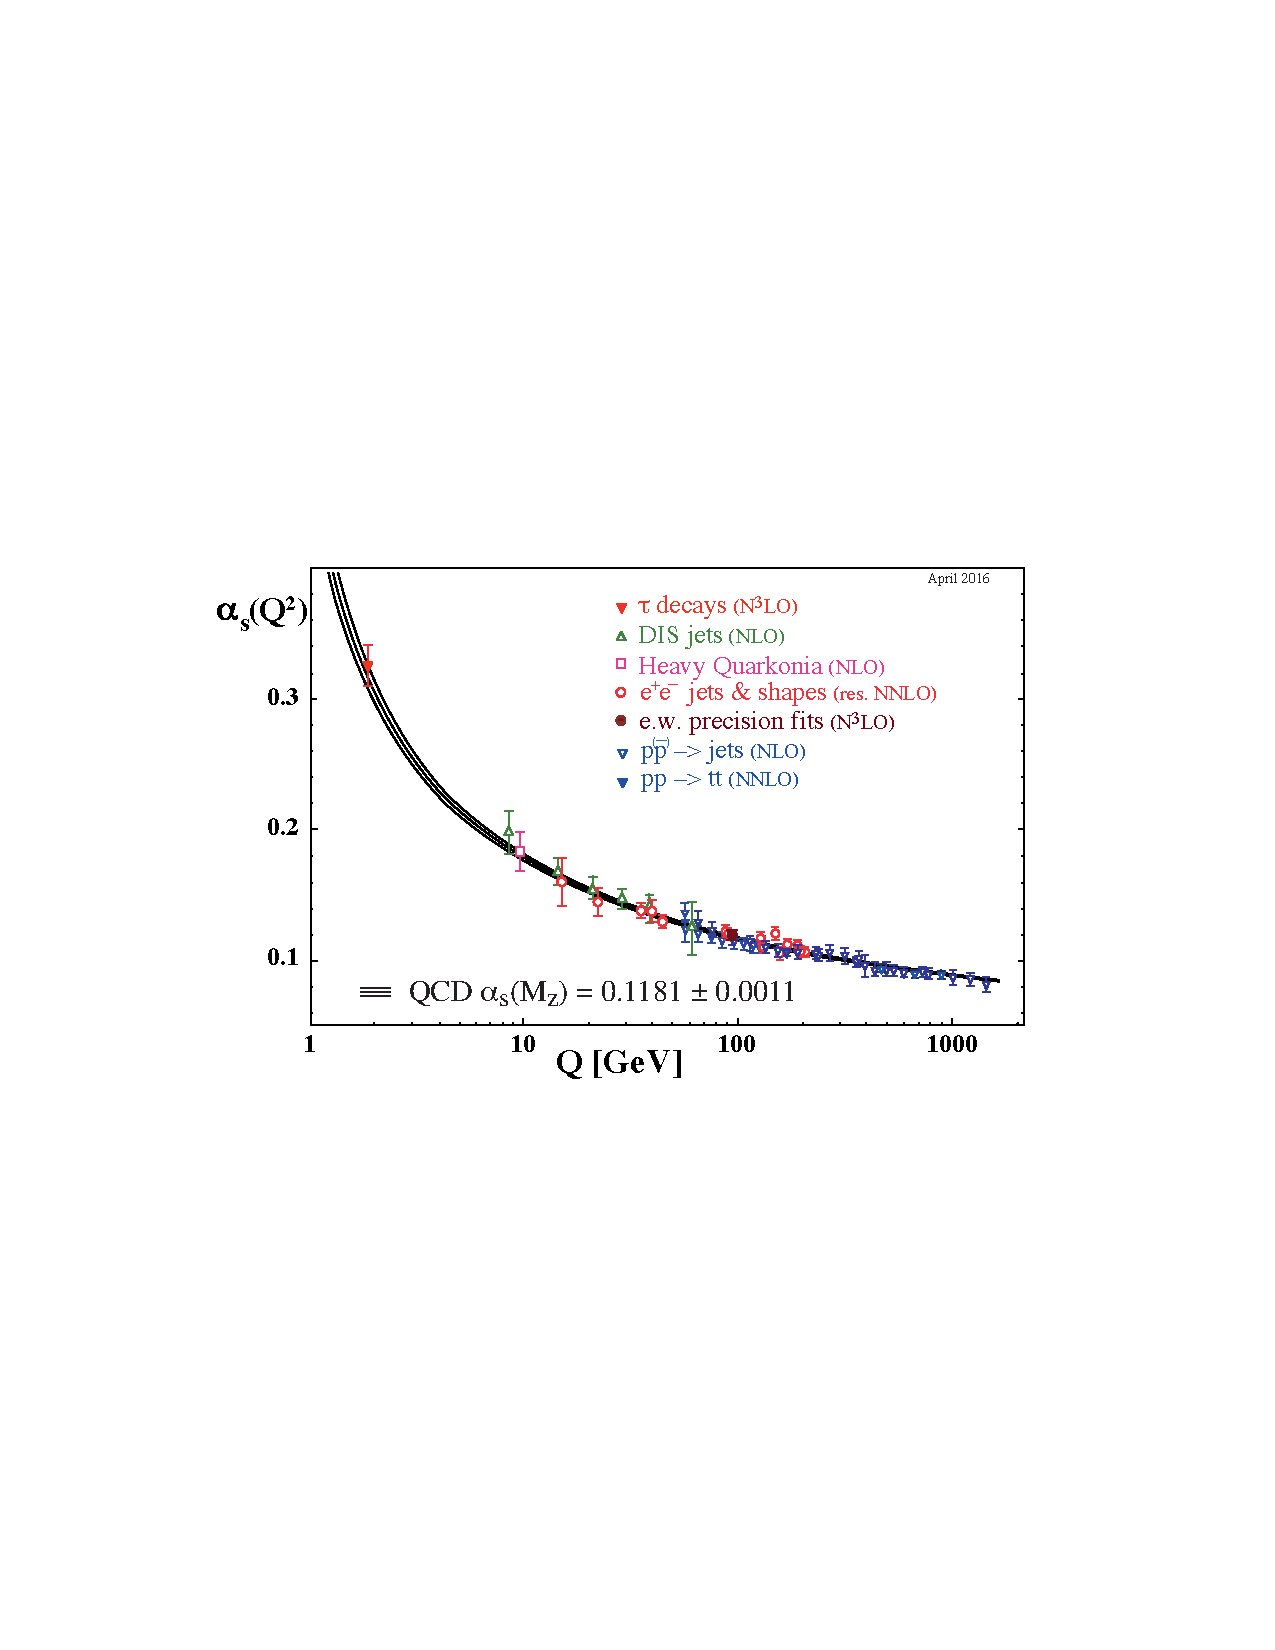
\includegraphics[width=0.7\linewidth]{img/theory/alphasscaling.pdf}
    \caption{
        Measurements of $\alphas(Q)$ at several values for $Q$.
        % 
        The black lines indicates the running of $\as(Q^2)$ when setting $\asmz$ to the current PDF world average, plus or minus its uncertainty.
        % 
        Taken from Ref.~\cite{pdg}.
        }
    \label{fig:alphasscaling}
  \end{center}
\end{figure}



% ____________________________________________________________________________
\subsection{The Higgs mechanism}

Experimental observations undeniably point to massive $\wboson$ and $\zboson$ bosons, but including naive mass terms in the Lagrangian manifestly violates local gauge invariance.
% 
The Brout--Englert--Higgs mechanism~\cite{Higgs:1964pj,Englert:1964et,Guralnik:1964eu} was originally introduced as a solution to explain the massiveness of the vector bosons without violating gauge invariance.
% 
This section shortly illustrates the principle of the Higgs mechanism in the SM, closely following the reasoning found in Ref.~\cite{Djouadi:2005gi}.
% 
Rather than looking at the SM, consider a Lagrangian with a complex scalar field $\phi = \phi_\mathrm{R} + \imag \phi_\mathrm{C}$ coupled to a gauge field $A_\mu$ that resembles a photon in the QED Lagrangian:
% 
\begin{linenomath*}
\begin{equation}
\label{eq:lagrangian-higgs}
\lagrangian =
    -\frac{1}{4} F_{\mu\nu} F^{\mu\nu}
    + (\partial^\mu - \imag e A^\mu) \phi^\ast (\partial_\mu + \imag e A_\mu) \phi
    - \underbrace{(\mu^2 \phi^\ast \phi + \lambda (\phi^\ast \phi)^2)}_{V(\phi)}
\,,
\end{equation}
\end{linenomath*}
% 
where $F_{\mu\nu} = \partial_\mu A_\nu - \partial_\nu A_\mu$ and $V(\phi)$ is a potential that yields a self-interaction for $\phi$.
% 
It can be easily verified that this Lagrangian is invariant under the transformations
% 
\begin{linenomath*}
\begin{equation}
\label{eq:transformations-higgs}
\phi(x) \to \exp{\imag \alpha(x)} \phi(x)
\quad \text{and} \quad 
A_\mu(x) \to A_\mu(x) - \frac{1}{e} \partial_\mu \alpha(x)
\,.
\end{equation}
\end{linenomath*}
% 
For $\mu > 0$, the term $\mu^2 \phi^\ast \phi$ is a regular mass term; the Lagrangian describes simply a `charged' scalar particle of mass $\mu$ and an `electromagnetic' field $A_\mu$, much like the QED Lagrangian for a complex scalar field except a $(\phi^\ast\phi)^2$ self-interaction is added.
% 
For $\mu < 0$, the minimum of the potential, found by solving $\partial V / \partial \phi = 0$, yields:
% 
\begin{linenomath*}
\begin{equation}
\left< 0 | \phi^\ast\phi | 0 \right> = \frac{-\mu^2}{2\lambda}  \equiv  \frac{v^2}{2}
\quad \left( \text{with} \; v = \sqrt{\frac{-\mu^2}{\lambda}} \right)
\end{equation}
\end{linenomath*}
% 
and the vacuum expectation value, $\left< 0 | \phi | 0 \right>$, becomes non-zero:
% 
\begin{linenomath*}
\begin{equation}
\left< 0 | \phi | 0 \right> = \sqrt{ \frac{-\mu^2}{2\lambda} } = \frac{v}{\sqrt{2}}
\,.
\end{equation}
\end{linenomath*}
% 
Clearly the Lagrangian can no longer be interpreted as that of a particle of mass $\mu$.
% 
In order to rewrite the Lagrangian so that the physical interpretation of massive particles is restored, $\phi$ is expanded around the vacuum expectation value:
% 
\begin{linenomath*}
\begin{equation}
\label{eq:expansion-around-minimum}
\phi = \frac{1}{\sqrt{2}} \left( v + \phi_1(x) + \imag \phi_2(x) \right)
\,.
\end{equation}
\end{linenomath*}
% 
Using the gauge transformations in Equation~(\ref{eq:transformations-higgs}) and a clever choice of $\alpha(x)$, the imaginary part of this expansion can be set to $0$:
% 
\begin{linenomath*}
\begin{equation}
\phi = \frac{1}{\sqrt{2}} \left( v + \phi_1(x) + \imag \phi_2(x) \right)
\to
\phi^\prime = \exp{i\alpha(x)} \frac{1}{\sqrt{2}} \left( v + \phi^\prime_1(x) \right)
\,.
\end{equation}
\end{linenomath*}
% 
As we will not use the untransformed fields any further, from here on the prime is omitted from $\phi_1^\prime$.
% 
The expansion is then inserted into the Lagrangian in Equation~(\ref{eq:lagrangian-higgs}).
% 
Performing the substitution is straightforward but lengthy; the derivation is given in Appendix~\ref{app:theory}, and here only the result is given:
% 
\begin{linenomath*}
\begin{equation}
\lagrangian \to \lagrangian^\prime =
    -\frac{1}{4} F_{\mu\nu} F^{\mu\nu}
    + \frac{1}{2} \partial^\mu \phi_1 \partial_\mu \phi_1
    + \frac{1}{2} e^2 (v+\phi_1)^2 A^\mu A_\mu
    - \frac{1}{4}\lambda\phi_1 - v\lambda\phi_1^3 + \mu^2\phi_1^2 - \frac{1}{4}\mu^2 v^2
\,.
\end{equation}
\end{linenomath*}
% 
The first two terms of the transformed Lagrangian look similar to the untransformed case.
% 
Additionally, there are $\phi_1^3$ and $\phi_1^4$ interactions, a constant term which is of no importance, and a mass term for $\phi_1$ that corresponds to particle of mass $-2\mu$.
% 
Expanding the third term yields the interactions between $\phi_1$ and $A_\mu$, but importantly, it also yields a term $\frac{1}{2}e^2v^2 A^\mu A_\mu$; this then is the mass term for $A_\mu$.
% 
The transformations described in Equation~(\ref{eq:transformations-higgs}) are clearly not valid if applied analogously to the fields in this transformed Lagrangian; the symmetry that was present before the transformation is, ostensibly, `broken'.


Spontaneous symmetry breaking in the SM Lagrangian is conceptually not different from the above demonstration, but significantly lengthier and slightly more complicated.
% 
Instead of a single complex scalar field, one considers a complex doublet of scalar fields, and carefully picks the vacuum around which to expand so the $U(1)$ symmetry of QED is preserved.
% 
The derivation of the transformed Lagrangian can be found in Ref.~\cite{Djouadi:2005gi}.
% 
In the end one finds massive $\zboson$ and $\wboson$ bosons, a massless photon, and a massive Higgs boson, with triple and quartic self-interactions much like in the derivation above.
% 
Also the fermion masses can be explained through the Higgs mechanism, and in the SM it turns out the fermion mass is proportional to the coupling of the Higgs boson with the respective fermion.
% 
Although the Higgs mechanism incorporates masses into the SM Lagrangian beautifully, the actual values of the masses need to be determined experimentally.



% ____________________________________________________________________________
\subsection{The Higgs production and decay modes}

While Higgs boson production and decay is in principle possible through a myriad of modes and channels, only few are relevant in the context of hadron colliders.
% 
As the rest of this thesis is concerned with Higgs boson couplings, also the basic scalings of the production modes and decay channels in terms of Higgs boson couplings is discussed briefly.


The Higgs boson is produced at hadron colliders through the following production modes (sorted by decreasing production cross section):
% 
\begin{itemize}
\item \textit{Gluon fusion} (\ggh), which in the SM exists only via a loop of (usually heavy) particles that couple to the Higgs boson, as the direct coupling of the Higgs boson to the gluon field is zero in SM;
% 
\item \textit{Vector boson fusion} (\vbf), in which the Higgs boson is radiated off a virtual vector boson; the final state is characterized by two jets in the forward regions;
% 
\item \textit{Associated production with a vector boson} (\vh), in which the Higgs boson is radiated off a non-virtual vector boson;
% 
\item \textit{Associated production with top quarks} (\tth), in which the Higgs boson is radiated off a top quark; and
% 
\item \textit{Associated production with bottom quarks} (\bbh), in which the Higgs boson is radiated off a bottom quark.
\end{itemize}
% 
The leading order diagrams for these production modes are shown in Fig.~\ref{fig:productionmodes}.
% 
The $\ggh$ production mode is dominant at the LHC, and its scaling in terms of Higgs boson couplings is complicated by interference terms.
% 
The $\tth$ and $\bbh$ production modes contain at leading order a single quark-Higgs boson vertex, which results in a simple quadratic dependence on the Higgs boson couplings for the respective production cross sections.


\begin{figure}[hbtp]
  \begin{center}
    \includegraphics[width=0.7\linewidth]{img/theory/productiondiagrams_combined.png}
    \caption{
        Summary of the dominant Higgs boson production modes at hadron colliders: $\ggh$ (top left), $\vbf$ (top right), $\vh$ (bottom left), and $\tth$ (bottom right).
        % 
        The $\bbh$ production mode has the same leading order diagram as $\tth$, but with the top quarks replaced by bottom quarks.
        % 
        Adapted from Ref.~\cite{productionmodes-grab}.
        }
    \label{fig:productionmodes}
  \end{center}
\end{figure}


The Higgs boson decay channels are slightly more numerous.
% 
The most common decay channels without a loop are the decays to two $\zboson$ bosons ($\hzz$), two $\wboson$ bosons ($\hww$), two $\taulepton$ leptons ($\htautau$), two $\bquark$ quarks ($\hbb$), and two $\cquark$ quarks ($\hcc$).
% 
The decay widths of these channels all scale quadratically with respect to their SM decay widths in terms of the respective coupling to the Higgs boson.
% 
For the fermions, the decay width at leading order is given by
% 
\begin{linenomath*}
\begin{equation}
\text{Get from Higgs Hunting}
\,.
\end{equation}
\end{linenomath*}
% 
Since the Higgs boson-fermion couplings are proportional to the fermion mass, the decay width is typically larger for heavier fermions, with the obvious exception of the decay width to two top quarks.
% 
In practice, the decay width for quarks lighter than the charm is negligible, as well as the decay width to two electrons.
% 
The leading order decay width to vector bosons is given by
% 
\begin{linenomath*}
\begin{equation}
\text{Get from Higgs Hunting}
\,.
\end{equation}
\end{linenomath*}
% 


Besides decays involving a single vertex, the Higgs boson decays via loops to two photons ($\hgg$), two gluons ($\hgluglu$), and a gluon and a $\zboson$ ($\hzg$).
% 
In these cases the decay width calculation needs to take interference terms into account.
% 
For example, in the case of $\hgg$, the decay width is given by
% 
\begin{linenomath*}
\begin{equation}
\text{Get from Higgs Hunting}
\,.
\end{equation}
\end{linenomath*}

\tk{Continue here, need Higgs Hunting.}



% ____________________________________________________________________________
\subsection{The Higgs boson couplings and the transverse momentum spectrum}

\tk{Include $\kappac$ results section?}



